\chapter{Database Design}
\thispagestyle{special}
\section{Attributes}
The database contains following tables:
\textbf{Users:}\\
     Username\\
  Password\\
\\
    \textbf{Companies:}\\
    Company Id\\
    Company Name\\
    Description\\
\\
    \textbf{Info:}\\
    no\\
    comp id\\
    suggestion\\
    no of rounds\\
    package\\
    project\\
    success\\
    failure \\
    \\
\section{ER Diagram}\\\
\textbf{}\\\
\centerline{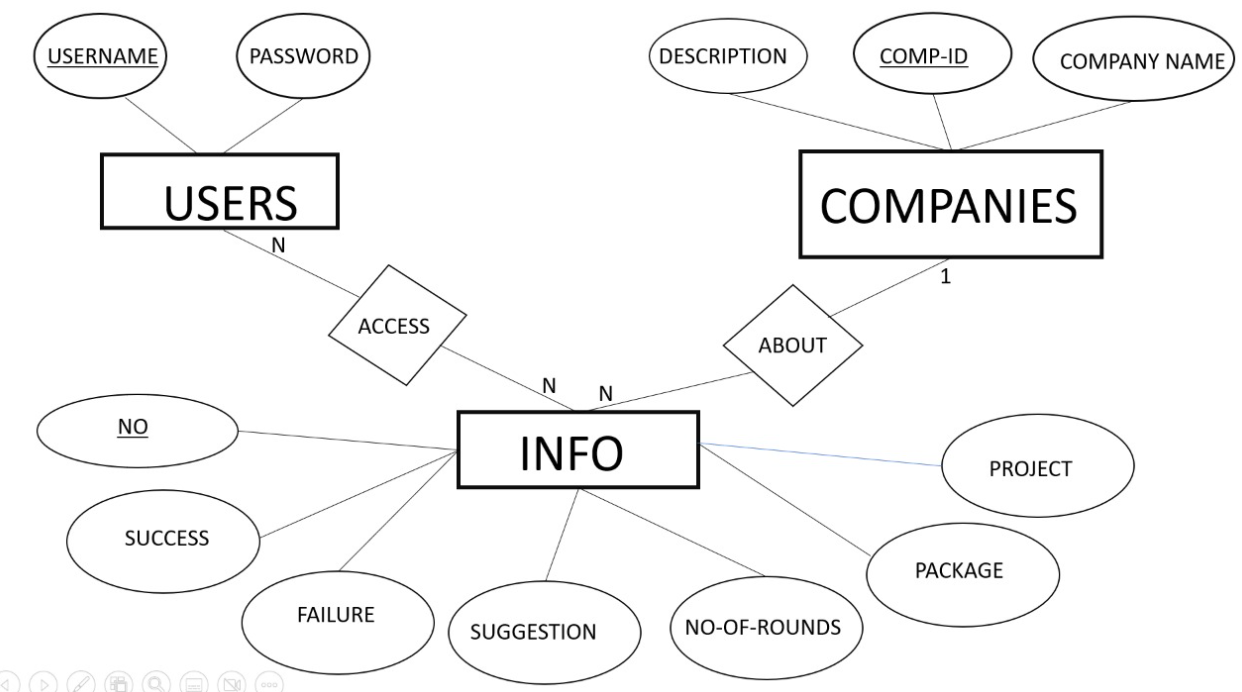
\includegraphics[scale=0.5]{ER-D.png}}\\\\\
		\end{figure}\\
 \textbf{}\\\ 
\centering{Fig.3.1. ER Diagram for Placement Management System}\\
\justifying{The Entity Relationship Diagram explains the relationship among the entities present in the database. ER models are used to model real-world objects and the relation between these real-world objects.ER Diagram is the structural format of the database.}\\ 
\justifying{ER Model is used to model the logical view of the system from a data perspective which consists of these symbols:
\begin{itemize}
    \item \textbf{Rectangles}: Rectangles represent Entities in the ER Model.
    \item \textbf{Ellipses:} Ellipses represent Attributes in the ER Model.
    \item \textbf{Diamond:} Diamonds represent Relationships among Entities.
    \item \textbf{Lines:} Lines represent attributes to entities and entity sets with other relationship types.
    \item \textbf{Double Ellipse:} Double Ellipses represent Multi-Valued Attributes.
    \item \textbf{Double Rectangle:} Double Rectangle represents a Weak Entity.
\end{itemize} 
\newpage
\textbf{Info about ER Diagram:} \\It consists of three Attributes mainly:- \\
Users\\
Companies\\
Info
\section{Relational Schema}
\centerline{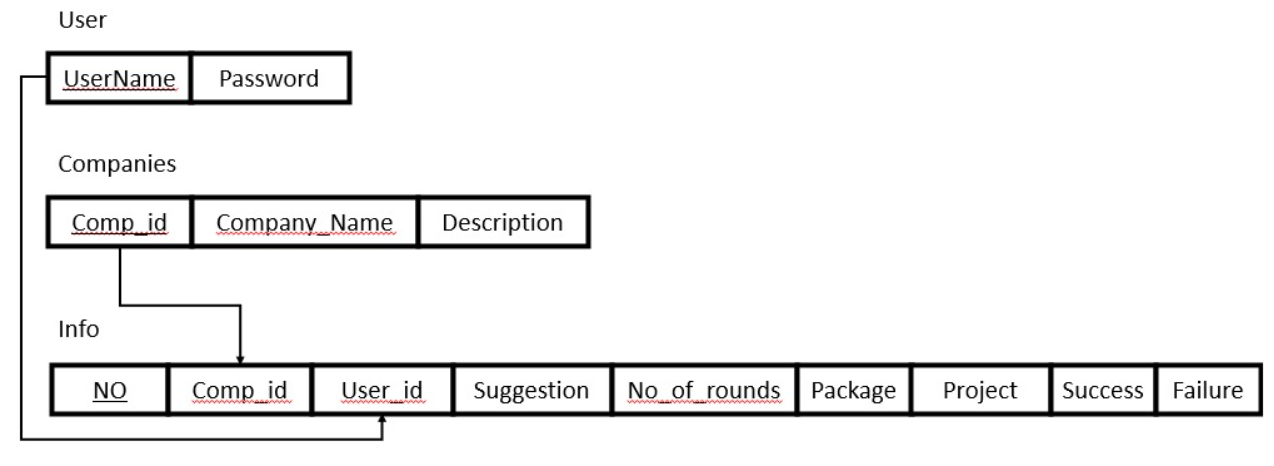
\includegraphics[scale=0.5]{schema.png}}\\\
		
  \centering{Fig.3.2. Schema Diagram for Placement Management System}\\
\justifying{A database schema is the skeleton structure that represents the logical view of the entire database. It defines how the data is organized and how the relations among them are associated. It formulates all the constraints that are to be applied on the data.A database schema defines its entities and the relationship among them. It contains a descriptive detail of the database, which can be depicted by means of schema diagrams. It’s the database designers who design the schema to help programmers understand the database and make it useful. } 
